% !BIB program = bibtex

\documentclass[12pt,letterpaper]{article}
\usepackage[utf8]{inputenc}
\usepackage[T1]{fontenc}
\usepackage{amsmath}
%\usepackage{amsfonts}
%\usepackage{amssymb}
\usepackage{makeidx}
\usepackage{graphicx}
\usepackage[normalem]{ulem}
\usepackage{subcaption}
\usepackage{float}
\usepackage{longtable}
\usepackage{multirow}
\usepackage{titlesec}
\setcounter{tocdepth}{2}
\usepackage[margin=1in]{geometry}
\usepackage{ntheorem}
\usepackage{booktabs}
\usepackage{dcolumn}
\usepackage[stable]{footmisc}
\usepackage{setspace}
\doublespacing
% font
\usepackage[charter,cal=cmcal]{mathdesign}
\usepackage{endnotes}
\let\footnote=\endnote

\usepackage{ntheorem}
\newtheorem{hyp}{Hypothesis}
\newtheorem{subhyp}{Hypothesis}[hyp]
\renewcommand\thesubhyp{\thehyp.\alph{subhyp}}
\usepackage{tikz}
\usetikzlibrary{arrows, decorations.pathmorphing, backgrounds, fit, positioning, shapes.symbols, chains, decorations.pathreplacing}
\usepackage[round]{natbib}
\bibpunct{(}{)}{;}{a}{}{,~}
\usepackage[space]{grffile}
\graphicspath{{./figures/}}
\usepackage[affil-it]{authblk}
\makeatletter

\def\@maketitle{%
	\newpage
	\null
%	\vskip 2em%
	\begin{center}%
		\let \footnote \thanks
		{\Large\bfseries \@title \par}%
		\vskip 1em%
		{\normalsize \today}%
	\end{center}%
	\par
	%\vskip 1.5em
	}
\makeatother

\title{Keeping Your Friends Close, But Acquaintances Closer: Why Weakly Allied States Make Committed Coalition Partners}

\begin{document}
	
\begin{singlespace}
\maketitle

\begin{abstract}
	Why do states join wartime coalitions despite the absence of a salient threat or strong ties to the coalition leader? We argue states make unexpectedly high contributions to coalition warfare as a costly signal of their desire for a stronger relationship with the coalition leader. Conventional theories insufficiently explain why states without immediate security interests or strong ties to the lead state over-contribute relative to their capacity. Using newly compiled data on troop contributions to the war in Afghanistan (2001-2014), we find states are most likely to contribute a higher share of their armed forces when their relationship with the US has unrealized alliance potential. States with under-performing alignments leave substantial room for subsequent gains to be had from signaling their commitment to the leading coalition actor. Our finding helps explain why states risk the costs of war -- casualties and domestic accountability -- by participating in coalition warfare.
\end{abstract}
\end{singlespace}

Word Count: 11,478

\newpage

\section{Introduction}
	In 2001 the United States launched the war in Afghanistan with the goal of overthrowing the Taliban and dismantling Al-Qaeda. But it did not do so alone; instead it led a coalition of 50 other states that fought alongside the United States until the war formally ended in 2014.\footnote{Operation Enduring Freedom (OEF) and International Security Assistance Force (ISAF) were two simultaneous missions in Afghanistan. The former was the initial US operation undertaken as part of the War on Terror. ISAF refers to the coalition operation under NATO command.} Every state's contribution differed. While the United States sent thousands of troops for the duration of the conflict, some European states contributed only a handful to fulfill their contractual alliance obligations under NATO. Other participants without formal alliance obligations incurred significant costs by sending troops. New Zealand, for example, lost almost a dozen troops in the Afghanistan conflict -- a difficult thing for a state leader to justify to their public when the outcome of the conflict is largely immaterial to the state at hand and when it has no contractual obligation to participate.

	This is exemplary of a broader trend in coalition warfare \citep{vonhlatky_greatasymmetryamerica_2010}. Some states contribute forces to coalition wars because they care about the material outcome of the conflict and hope to influence that outcome in some significant way. Others contribute forces because alliance obligations or expectations create a cost to free riding. But what motivates some states to pay a heavy cost to fighting alongside another country when traditional security calculations or alliance obligations don't apply? Neither of those theories explain contributions like that of New Zealand to the war in Afghanistan; states that are unaffected by the outcome of the conflict, that have no notable ability to influence the outcome of the war, that experience no reputational cost from refusing to participate, and yet willingly risk high costs from their participation.
	
	Many of the states that contributed the highest share of their armed forces to ISAF, including New Zealand, were not those anticipated by conventional theories. Of the 10 states that committed the largest share of their military forces to the theater at the start of the war, only Turkey is geographically proximate and only 5 of the 9 non-US countries were NATO members. And although every NATO member participated in at least some capacity, over a half dozen had no physical presence in Afghanistan until more than halfway through the mission.

	This paper explains such contributions by developing a new theory about coalition warfare participation by states whose primary objective in fighting is not to influence the outcome of the conflict or fulfill the role expected of close and reliable allies. Instead, states contribute forces to coalition warfare in order to \textit{become} close allies by developing a reputation for reliability and effort. These states make costly contributions not because they already have close relationships with the coalition leader, but because their relationship has \textit{unrealized alliance potential}. As such, their contribution is disproportionately costly in order to signal their desire for a stronger relationship with their coalition partner. We find that if state military contributions are measured as a share of what they theoretically could have contributed -- the number of troops they deployed relative to the size of their armed forces -- then the highest contributions are most likely to come from states with an interest in developing a stronger relationship with coalition leaders. In other words, states that wish to increase the strength of their relationship with states leading a coalition do so by sending a larger and more costly portion of their armed forces than states whose participation was expected given formal obligations or a highly salient threat.
	
	We test our theory using new data on each country's relative annual contribution to the Afghanistan war as well as each country's latent relationship strength with the United States. Unlike prior analyses that focus on absolute troop contributions, we consider the cost of each state's contribution as a ratio of troops deployed relative to the size of a country's armed forces. If a small state is trying to signal to the coalition leader that it is willing to overexert itself on behalf of that coalition leader, then relative contributions matter most. Rather than being a function of one's current relationship to the coalition leader, the cost of one's contributions are instead shaped by the discrepancy between the closeness of their current relationship and the relationship they could have, but that has not yet been realized. This better identifies the group of states that, like New Zealand, may over-contribute in order to improve the closeness of the current relationship. Our analysis confirms that states whose security relationship with the US is weaker than it should be, given the alignment of their respective security interests, contributed a larger share of their armed forces to the US-led war in Afghanistan (ISAF).
	
	This finding has important implications for understanding not only how states fight, but also the costly means by which states seek to re-align themselves in international alliance networks. Conflict is generally understood as a costly tool which states employ to achieve their international objectives \citep{betts_shouldstrategicstudies_1997}. Yet those objectives can be unrelated to the outcome of the conflict itself. Simply put, war can be a good excuse for improving ties with like-minded states. States are willing to incur costs in an institutional context not when they are already well-embedded in those institutions, but when they have the most to gain from further institutionalization.

	This paper proceeds in five parts. In part two, we explore existing explanations for coalition warfare, which thus far have focused on the decision to join coalition efforts rather than the extent of their participation. Part three develops our theory by applying a costly signaling theory to coalition warfare through a novel measure of the costliness of a state's contribution to coalition warfare: the relative pressure of that mobilization based on the size of its available armed forces. Part four empirically test this finding by examining coalition contributions during the war in Afghanistan (2001-2014), which presents a ripe test case for our theory given variation in the alliance obligations of the states that participated as well as their level of participation. Section five includes a discussion of the generalizability of our results for the broader theory, explaining how states seek to alter and leverage their position within the network of capable international actors. Section six concludes.

\section{Existing Theories of Coalition Warfare Contributions}
	An alliance between two actors constitutes a promise to take a certain action in the event of a particular contingency \citep[526]{altfeld_decisionallytheory_1984}. In the international security context, an alliance is thus often a promise to defend the other actor in the event of a threat to their security \citep{waltz_theoryinternationalpolitics_1979, walt_originsalliance_1987} or to facilitate mutually beneficial cooperation when states have common objectives \citep{keohane_hegemonycooperationdiscord_1984, wolford_showingrestraintsignaling_2014}. Although the importance of theorizing differing contributions has been recognized in the context of US-led coalition efforts, this work has focused on single-dyad case studies. Scholars have recognized that these efforts would benefit from broader analysis that tests the generalizability of their findings \citep[4-5]{mello_politicsmultinationalmilitary_2018}. Attempts to explain why countries contribute to alliances to varying degrees can be divided into four different categories; theories of collective action, the balance of threat, alliance dependence, and domestic politics \citep{bennett_burdensharingpersiangulf_1994, haesebrouck_democraticparticipationair_2016}.
	
	The \textit{collective action hypothesis} introduced by \citet{olson_economictheoryalliances_1966} posits that dominant states will end up making the largest contributions to alliances because smaller states can simply free ride while continuing to garner the benefits of the alliance relationship writ large. These dominant states, with larger economies and militaries, end up paying a disproportionate burden to secure goods even when the public benefits of those goods are reaped by states that made little contribution themselves. The \textit{balance of threat hypothesis} argues that state contributions should be proportional to the gravity of the threat an issue presents to a state. When faced with a larger threat, a state will contribute more to an alliance coalition that they expect can mitigate that threat \citep{walt_originsalliance_1987, baltrusaitis_coalitionpoliticsiraq_2010, sandler_natoburdensharing_2014}. The \textit{alliance dependence hypothesis} argues that states in an alliance must balance two competing fears; the fear of abandonment and the fear of entrapment \citep{snyder_securitydilemmaalliance_1984}. Problematically, reducing one of these risks necessitates an increase in the risk of the other. Allied support is thus explained by how a state feels about these relative risks; states will contribute to an alliance when the fear of abandonment exceeds the fear of entrapment. States that most fear abandonment will be those that are most dependent on the other partner in the alliance because the military and economic payoffs of the alliance relationship would be difficult to replace. This theory has been expanded by scholars who note that ``alliance value" explains contributions by states who believe they can leverage relationships with current allies in their favor \citep{davidson_neoclassicalrealistexplanation_2011}. \textit{Domestic hypotheses} of alliance contributions take multiple forms \citep{,tago_whenaredemocratic_2009, ashraf_politicscoalitionburdensharing_2011, pilster_aredemocraciesbetter_2011, wolford_nationalleaderspolitical_2016, mello_pathscoalitiondefection_2020}. Theories of state autonomy and domestic society predict that leaders that can insulate themselves from external constraints on their decision-making about alliance contributions are consequently able to do so even when these leaders' preferences regarding contributions differ from those of the public \citep{saideman_ambivalentcoalitiondoing_2016, vonhlatky_ideologyballotsalliances_2018}. Theories of bureaucratic politics instead examine the relationship within the government. Bureaucratic decision-making requires negotiations and bargaining among relevant actors and as such state contributions are the outcome of these bargaining decisions and the environment shaping the bargaining framework \citep{rathbun_partisaninterventionseuropean_2004, mello_democraticparticipationarmed_2014, mello_pathscoalitiondefection_2020}. It is not just about the ideological position of a state leader, but how that interacts with the ideological position of the opposition party and the way state leaders navigate that as the domestic situation changes \citep{mello_pathscoalitiondefection_2020}.\footnote{\citet{mello_pathscoalitiondefection_2020} looks at the domestic causes of a state's decision to \textit{withdraw} from a coalition conflict, rather than whether to contribute in the first place.}

	Other literature on state contributions to joint efforts have examined distinct, but related multilateral efforts like UN peacekeeping. In this context, state contributions are influenced by network centrality \citep{dorussen_networkedinternationalpolitics_2016}, international factors \citep{mullenbach_decidingkeeppeace_2005}, geostrategic interests \citep{baltrusaitis_friendsindeedcoalition_2008}, regime type \citep{lebovic_unitingpeacedemocracies_2004}, and side payments and issue-linkages \citep{henke_networkedcooperationhow_2019}. While theoretically important, these findings do not explain the costliness of a state's contribution nor whether that contribution was used as a signal to improve a state's ties with other actors in the network. Their network position is assumed as a static factor explaining the level of contribution when in reality it is a position that states want to actively manipulate. The costliness of UN peacekeeping contributions as a signal is also harder to measure considering the lower risk of casualties and collateral damage. Domestic audiences  also are less attuned to their state's participation in UN peacekeeping than active military operations \citep{lehmann_publicperceptionspeacekeeping_1995}. 

\section{A Theory of Joint Coalition Warfare as a Costly Signal}
	Why do states cooperate with one another on security issues and how do states shore up and maintain that cooperation? Though there is extensive literature on the ways in which states aggregate their capabilities to bolster their security against foreign threats \citep{waltz_theoryinternationalpolitics_1979, walt_originsalliance_1987, morrow_alliancesasymmetryalternative_1991, conybeare_portfoliodiversificationmodel_1992}, the security benefits of an alliance do not precisely map onto the security benefits of joining a wartime coalition because coalitions and alliances are not synonymous. Coalitions can be a manifestation of an alliance promise or be an ad hoc relationship oriented toward an immediate goal rather than a broader security arrangement \citep[115]{weitsman_wartimealliancescoalition_2010}. Scholars have argued that because alliances are public goods, the benefits of the alliance can be reaped even if a member does not participate in an alliance's coalition efforts \citep{olson_economictheoryalliances_1966}. And yet, national defense is a club good, not a pure public good, because the protection benefits of an alliance can be excludable and rival \citep[336]{sandler_clubtheorythirty_1997}. After the end of the Cold War, the US leveraged NATO's security benefits via threats of exclusion to encourage risk-sharing and minimize free riding \citep[324-325]{ringsmose_natoburdensharingredux_2010}. As a result, states within security alliances must avoid the temptation to free ride because doing so risks losing the benefits of alliance membership. States thus have to devote resources to maintain the receipt of these club goods and can do so by demonstrating what they bring to the table. For example, President Trump's rhetoric regarding NATO burden-sharing has resulted in conversations within Canada about how to avoid the perception that they are free-riding on US security commitments \citep[143]{mckay_whycanadabest_2018}. So paradoxically, although the public good view of alliance holds that their benefits can still be accrued without participating in coalitions, the club good view identifies how participating in coalition efforts can increase the benefits of an alliance for any one member.
	
	This highlights the importance of identifying and theorizing the relationship between alliances and coalition efforts. In coalition efforts, unlike alliance more broadly, there are more clear private benefits to participating states. Advocates of the balance of threat perspective point to private incentives actors have to ensure that the aggregate contributions to defense are sufficient to deal with the threat \citep{bennett_friendsneedburden_1997, baltrusaitis_coalitionpoliticsiraq_2010, davidson_neoclassicalrealistexplanation_2011}. This private goods theory of coalition conflict, as distinct from alliances, explains why states would vary in the \textit{degree} of their contribution. Acquaintances make a costly contribution when they could have chosen to free ride not because their interest is in the public good of security achieved via victory in the conflict but rather because of their private interests vis-a-vis the state to whom they sent a costly signal of support like a security umbrella down the road or closer economic or diplomatic ties \citep{long_defensepactsinternational_2003}. Previous literature has noted that you should get a payoff from signaling that you honored an alliance commitment and states that do so get more allies in the future because they are seen as reliable \citep[427-428]{gibler_costsrenegingreputation_2008}. This is consistent with our logic where you hope that your signal of strongly valuing the relationship causes the other actor to later take actions that recognize that.
	
	Our theory thus lies at the intersection of research on coalitions and alliances to explain why states contribute more or less to coalitions than we would expect \citep{saideman_ambivalentcoalitiondoing_2016}. States get private goods from coalition war-fighting. For some states, that private good is a desirable war outcome. For others, the private good to be gained from coalition war-fighting is improving the quality of your relationship with the central actors leading that conflict. Participating in the war efforts of similarly aligned states is one way states can signal that they are not free riding on the relationship and are instead participating in burden sharing because they value the reciprocal and mutually-beneficial alliance commitments \citep[225-227]{maskaliunaite_sharingburdenassessing_2014}. This costly signal is conveyed when a state has over-contributed relative to the contribution that would be expected given their military capacity. Since alliances are a costly signal of one's intention to cooperate, it should also be true that fulfilling alliance-like obligations even when you are not bound by those alliance obligations would also be a signal of your desire to cooperate more in the future \citep[704]{warren_geometrysecuritymodeling_2010}. 

	\subsection{New Conceptions of Contribution Cost and Dynamic Interstate Alliances}
		We depart from current explanations of state contributions to coalition war efforts in how we conceptualize and empirically identify that contribution. The extent to which a country participates in a coalition war effort is distinct from whether they participate at all. The foundational literature on theories of collective action, the balance of threat, and alliance dependence typically examine whether a country participated; only domestic explanations focus on constraints regarding the \textit{extent} of contribution \citep{bennett_burdensharingpersiangulf_1994, bogers_missionafghanistanwho_2013, mello_pathscoalitiondefection_2020}.

		Contrasting findings among the first three theories are explained by examining the extent of state contributions rather than just whether they contributed \citep[4]{cranmer_coalitionqualitymultinational_2017}. Yet previous work examining the extent of state contributions still suffers from a biased conceptualization. Almost all prior analysis has measured a state's contribution in absolute terms; the number of troops, financial contributions, foreign aid, or peacekeepers sent to a particular operation \citep{mello_democraticparticipationarmed_2014, haesebrouck_explainingmemberstates_2016}. This measure makes sense for theories interested in explaining who contributes the most, since absolute terms describe the highest contributors \citep[40-41]{bogers_missionafghanistanwho_2013}. But absolute contributions do not tell us whether a state's contributions were more or less than expected nor does it tell us the relative cost of that contribution for the state in question \citep{kreps_eliteconsensusdeterminant_2010}. It is less costly for Great Britain to send 1,000 forces into a conflict theater than for Poland to do the same since Poland's comparatively small military force makes that mobilization an unusually large undertaking. Great Britain has a substantially larger military force and thus experiences a lower national cost in terms of the burden such a contribution places on its military forces and the zero-sum trade-off of this contribution relative to other security or financial needs. Absolute contributions thus do not reflect the cost of contributing; they instead represent the size of the state. Figure \ref{fig:measure_comparison_contribution} shows that a measure of a state's absolute contribution (here the percent of \emph{all states'} troops that are deployed in Afghanistan) provides different rankings of costliness than the percent of a state's relative contribution (the percent of \textit{that state's} troops that are deployed in Afghanistan). Just because a country has a large military -- France, for example -- does not mean it contributes a large percentage of its troops. Indeed, measuring contributions as the percent of a state's armed forces demonstrates that countries like Denmark, Estonia, Canada, and New Zealand participated in the conflict to a surprising extent. Measuring troops contributed as a ratio of other baselines like population size or GDP yield similar results \citep[41]{bogers_missionafghanistanwho_2013}.

		\begin{figure}[p!]
			\centering
			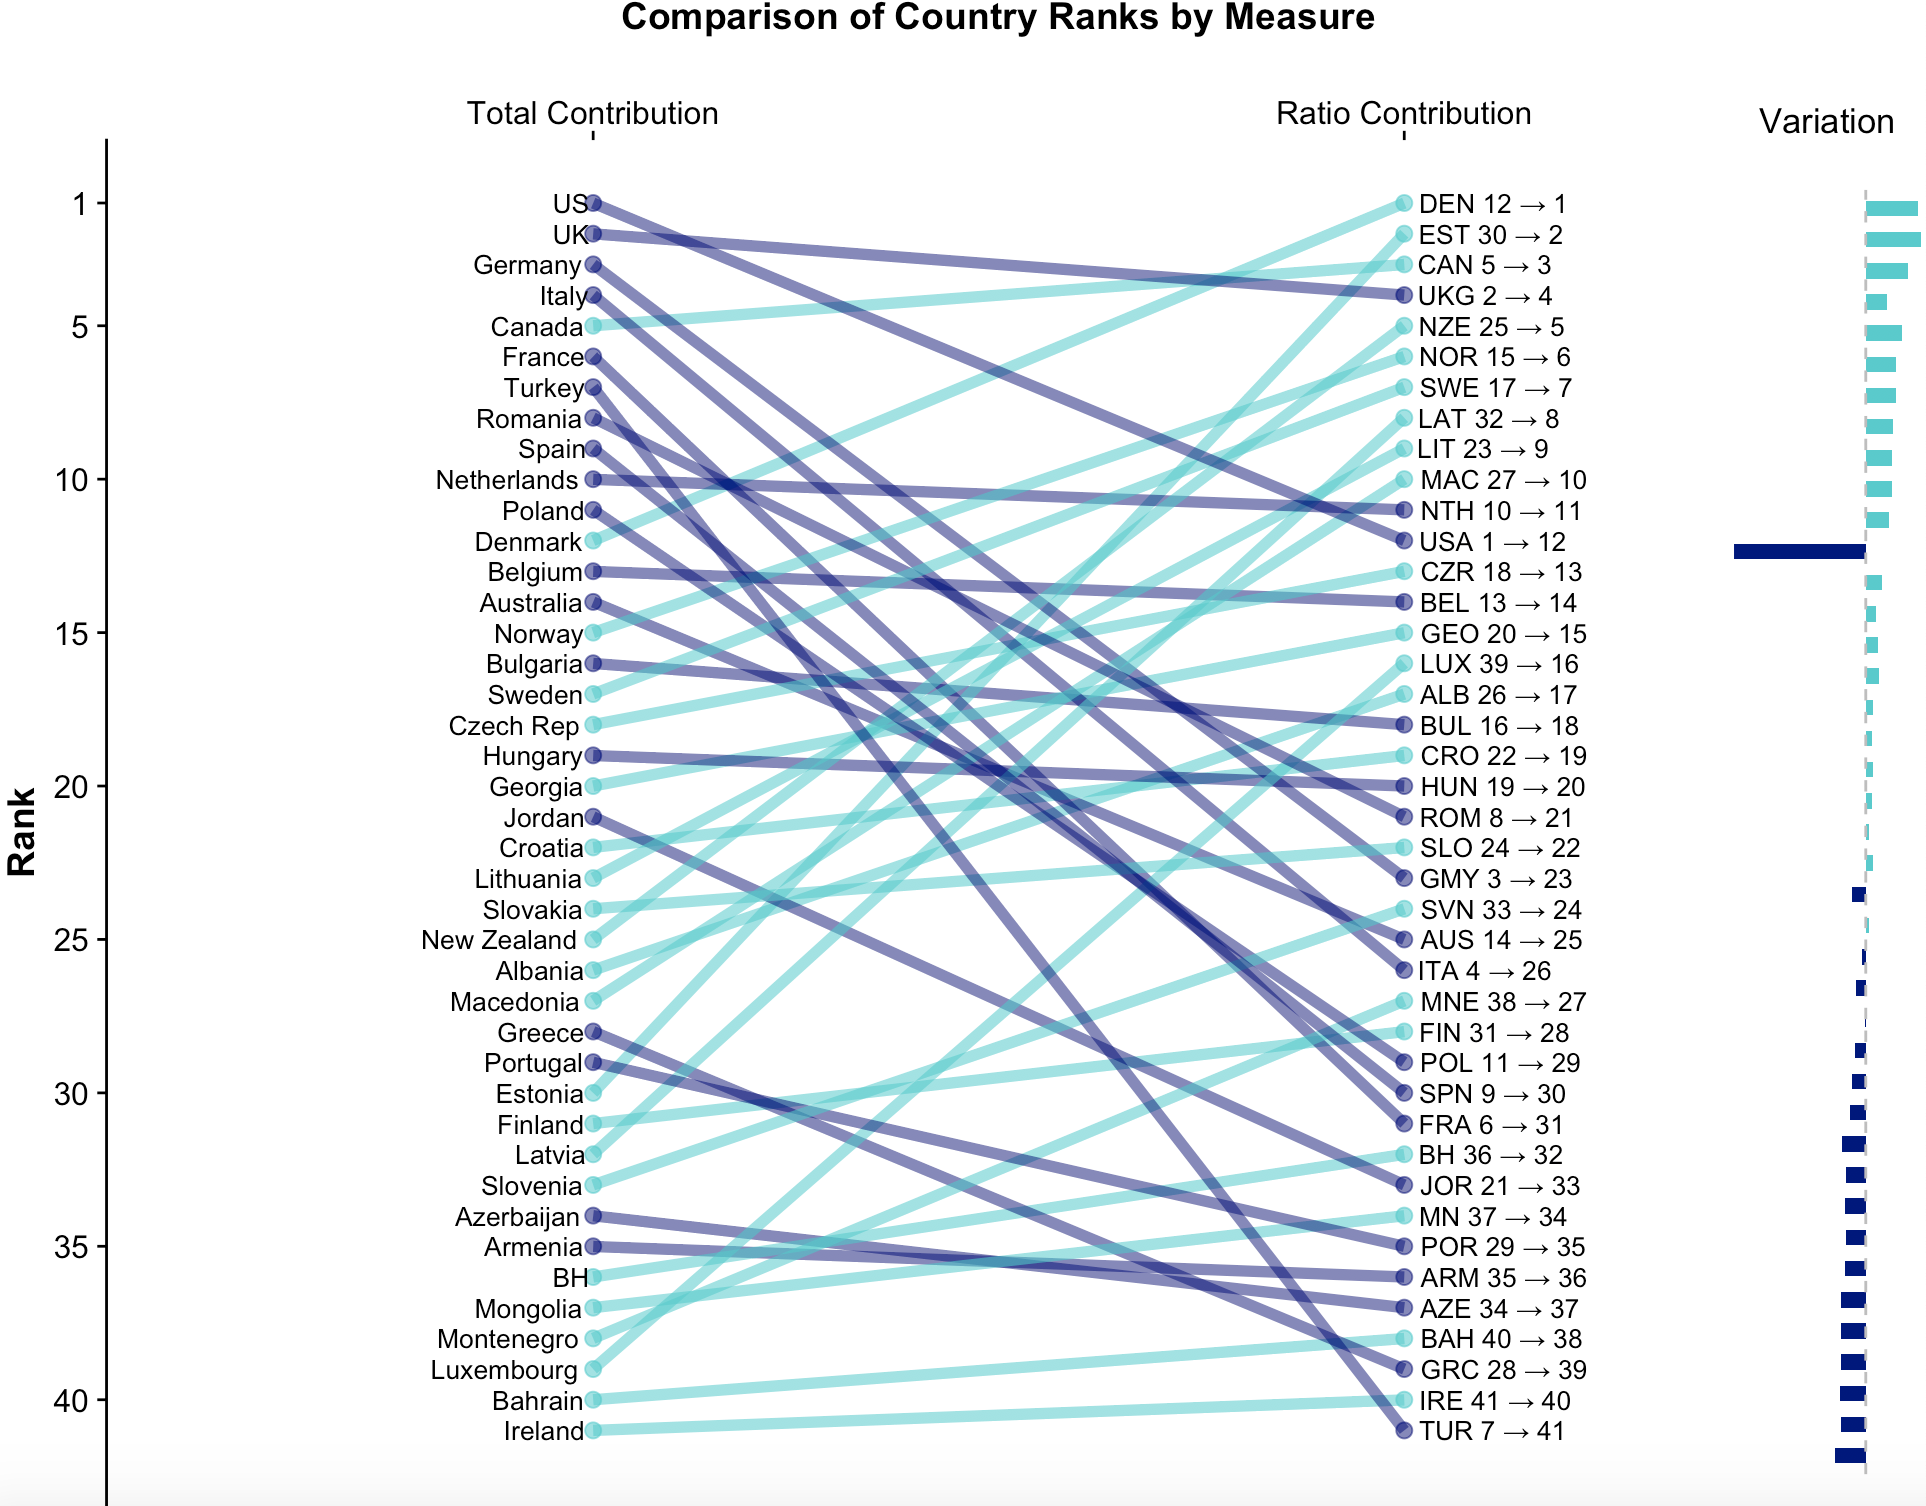
\includegraphics[width = \textwidth]{figures/contribution_slopeplot.png}
			\caption{Each column represents the ordinal rank of country contributions to the war in Afghanistan by number of troops. Dark blue lines indicate a country that is ranked higher in Total Contribution (left) than Ratio Contribution (right). Light blue lines indicate the inverse. The change in rankings per state are provided as well as the variation in rank change across the two measures. We hypothesize that states with unrealized alliance potential will have higher Ratio Contribution irrespective of their Total Contribution.}
			\label{fig:measure_comparison_contribution}
		\end{figure}

		The second problem is how current theories think about alliances. Conventional explanations anticipate the highest contributions coming from states that are dependent on the security guarantee of the central coalition actor and those that believe they have a special relationship with the United States \citep{graeger_revivalatlanticismnato_2009, biehl_strategiccultureseurope_2013, howorth_securitydefencepolicy_2014, haesebrouck_democraticparticipationair_2016}. However, this views the alliance relationship as static and oriented towards maintaining continuity in the current relationship rather than being forward-looking and seeking change. The conclusion is that countries that fight together do so because of their closely aligned interests.\footnote{Previous work by \citet{kreps_whendoesmission_2008} and \citet{henke_politicsdiplomacyhow_2017} has examined this issue from the perspective of the coalition leader.} This misses how fighting together can be a method for \textit{altering} the perceived alignment of interests rather than simply reflecting it \citep{weitsman_wagingwaralliances_2013}.
		
	\subsection{Benefits of Over-contributing Forces}
		The most costly contributions do not come from those with the strongest ties to the coalition leader \citep{ringsmose_natoburdensharingredux_2010, wolford_showingrestraintsignaling_2014}, those who care about their broader international reputation \citep{pedersen_bandwagonstatuschanging_2018}, or those who are capitulating to demands from the coalition leader \citep{schweller_newrealistresearch_1997}. Rather, over-contributing is a way to send a separating signal that even though a state is not closely aligned with the central actor prior to or at the outset of the conflict, it is willing to incur costs for the sake of the central actor in the hopes that it will realize that yet-untapped closer alignment. That closer alignment may be valued inherently, for unspecified reasons, or to help the state acquire side payments or policy concessions on unrelated issues.

		Costly over-contributions are an alliance signaling function under two conditions. First, the over-contributing state must have unrealized alliance potential, meaning the current depth of their alliance commitments does not adequately reflect the depth the alliance \textit{should} have given the alignment of the states' interests. While the conventional alliance hypotheses argue that the highest contributions will come from states that have a special relationship with the United States or those that are currently dependent on the security guarantee, we argue instead that a different set of states -- those that could have a more tightly linked relationship with the United States -- will make more costly contributions. States that already have a special relationship or a reliable security guarantee do not need to over-contribute because their relationship is, in a sense, locked-in. These states have some flexibility in their expected contributions and are unlikely to lose their special relationship status simply because they did not go above and beyond in contributing to the coalition effort. They just need to contribute enough that they are not seen as free riding. 

		We use a latent measure of alliance depth in order to identify the current depth of a state's alliance with the United States. By identifying this latent measure, we are able to differentiate correctly predicted alliance ties from those that are unanticipated. Given the close similarity in foreign policy preferences, the deep alliance relationship between the US and the UK is not surprising. The non-existence of any US-Venezuela security alliance is similarly predictable if a hunch was made based on the misalignment of those states' foreign policy preferences. We would not expect either the UK or Venezuela to be dissatisfied with the current state of their security alliance with the US even though one relationship is ``special" while the other is nonexistent. Our focus is thus states like New Zealand that don't fit this category. New Zealand -- despite historically consistent interests with the US regarding intelligence and security threats -- has a weak, informal, and largely ad-hoc security relationship with the United States \citep{fruhling_anzusreallyalliance_2018}. In statistical terms, our theory concerns the residual -- the gap between the expected alliance strength and observed alliance strength. States with a high residual between the predicted alliance depth and observed alliance depth are more likely to over-contribute troops as a signal of their interest and commitment to reducing that residual.
		
		Second, the leading state must perceive the contributing state's effort as occurring for the leading state's benefit. For an over-contribution to be a costly signal of one's commitment to their ally, the private incentives to contribute cannot just be egoistic security \citep{davidson_americaallieswar_2011}. If the contributing partner garners substantial private security benefits from participating in the war effort, the central coalition actor will be less likely to interpret the over-contribution as a signal of good will and may instead interpret it as a self-interested intervention that would have occurred irrespective of its benefits to the coalition leader \citep{tago_whystatesjoin_2007, lake_hierarchyinternationalrelations_2009, chapman_securingapprovaldomestic_2011}. Because the value of the signal is determined by its cost, not by its effect, it does not matter if the signaling state sends forces that can materially influence the outcome of the conflict \citep{davidson_americaallieswar_2011}. It only matters that the signal is interpreted as one that was costly for the sender irrespective of its impact on the war's outcome. In most cases, the powerful state not only does not need support from smaller states in order to win the conflict, it may actually want to maintain control of the forces that will determine the conflict outcome.  As a result, smaller states do not want to make contributions that are too influential in the conflict's outcome because of the risk of intruding upon the powerful state's decision-making. Importantly, this differs from other perspectives like \citet[72-75]{bennett_burdensharingpersiangulf_1994} and \citet{henke_buyingalliespayment_2019} since the US is not exercising leverage over smaller states to induce their contributions; instead the momentum comes from the smaller initiative-taking states whose contribution does more to serve their long-term interests than the immediate interests of the coalition leader.

		Based on this theory of costly contributions, what predicts what states will over-contribute troops to a coalition war effort because of the signal they hope to send to the coalition leader? Suppose one knew the degree of interest alignment between two actors and used that information to estimate the true depth of their relationship. In some cases, that estimate would be highly accurate; actors with highly aligned interests have deep relationships while those with misaligned interests have shallow or non-existent relationships. That estimate could err in two directions. First, the error could represent cases where a shallow alignment relationship is predicted, but the two actors are in reality quite close. Second, the error could represent cases where a deep alliance relationship is predicted but is not present. This error represents our independent variable. Cases where a close relationship is predicted but not observed represent unrealized alliance potential.

		\begin{hyp}
			A state with unrealized alliance potential with a coalition leader will make more costly contributions to that state's coalition conflicts than a state that is satisfied with its current security alliance.
		\end{hyp}

		Our theory thus predicts a positive relationship between a state's latent alliance potential with the central coalition actor and that state's expected cost of contributing to the coalition war effort. The allies already optimally aligned with the central coalition actor are not the states that make the highest relative contributions since they have no incentive to incur the unnecessary costs that high relative contributions entail. Instead, those that have an opportunity to become closer allies, relatively speaking, contribute the most.

\section{Research Design}
	\subsection{Data}		
		Our dependent variable is the extent of a state's contribution to the war in Afghanistan, which we measure using data on country-year troop contributions. Rather than relying on a raw measure of the number of troops a country sent to Afghanistan, we measure the cost of a contribution as the share of a state's armed forces that they deployed to Afghanistan in a given year. By measuring a state's contribution as the \emph{percent} of its total troops rather than the \emph{number} of troops we are able to measure the costliness of a state's contribution in a way that better differentiates states. We use troop count rather than military spending because of difficulties calculating the financial cost of conflict \citep{stiglitz_estimatingcostswar_2012}. This financial uncertainty makes an analogous measure of military spending in Afghanistan as a ratio of total military spending a difficult and unreliable metric for the dependent variable \citep{bruck_economiccostsgerman_2011}. Nonetheless, troop contributions and the financial cost of a country's participation should be sufficiently correlated because ISAF operated under NATO's principle of ``costs lie where they fall" meaning each state was responsible for the cost of their own troops.
		
		Data on each country's annual troop contributions and their overall military personnel were collected from the International Institute for Strategic Studies (IISS) Military Balance reports from 2002 -- 2015 \citep{internationalinstituteforstrategicstudies_militarybalance_}.\footnote{The reports publish data on the prior calendar year's activities.} Military personnel and deployment data from IISS has been used widely by previous scholars \citep[e.g.][]{walter_buildingreputationwhy_2006, rovner_hegemonyforceposture_2014, beckley_emergingmilitarybalance_2017, henke_politicsdiplomacyhow_2017} and unlike other sources used for the war in Afghanistan, benefits from coverage over the course of the entire war. We also conducted our analysis using the official ``NATO placements" which provide data on military contributions every few months, but they are not our primary data source since they only cover 2007--2014 and at irregular intervals. Nonetheless, the NATO placement deployment data and IISS deployment data correlate at 0.86 for the time period they both cover, validating the quality of the data used in the model.
		
		There are a variety of ways to measure burden sharing, including the number of troops as a share of population size, armed forces size, armed forces in the coalition, and GDP \citep[668-669]{hartley_natoburdensharingfuture_1999}. The costliness of a state's contribution is measured as a share of the size of their armed forces as opposed to GDP or military spending since the risk of casualties and collateral damage are two costs unique to personnel contributions that states are attentive to when deciding whether and to what extent they should participate in coalition warfare \citep{ringsmose_natoburdensharingredux_2010, chivvis_topplingqaddafilibya_2014, vonhlatky_cashcombatamerica_2015, haesebrouck_natoburdensharing_2017}. This measure thus best captures the security burden a country has willingly undertaken to fight in another state's war. We do not distinguish between the type of troop or whether they were in an active combat zone because of the unreliable or classified nature of that data \citep[44-45]{bogers_missionafghanistanwho_2013}.\footnote{An explanation of the origins of these national caveats in the Afghanistan mission is provided by \citet{saideman_comparingcaveatsunderstanding_2012}.} States may have only imprecise ex ante estimates about whether their troops are in a combat zone. Furthermore, countries like Canada tried to disguise whether their troops in Afghanistan were fulfilling only logistical support missions to mitigate domestic backlash from the public and from legislators \citep{reportprogresssecurity_2010}. While military tacticians may interpret troops sent to a combat zone as a more costly contribution than those sent elsewhere, national politicians -- the intended recipients of that signal -- are less likely to meaningfully make that distinction.

		Our independent variable is unrealized alliance potential with the United States. A state's alliance potential is measured by its preference similarity with the United States in United Nations voting patterns \citep{gartzke_preferencesdemocraticpeace_2000}. We operationalize the current strength of a state's alliance by replicating, temporally extending, and standardizing the \citet{benson_assessingvariationformal_2016} measure of alliance depth. This refers to the extent to which the alliance induces costs beyond wartime commitments. The resulting measure is a composite of whether an alliance requires: peacetime military contact, coordination of a common defense policy, integrated military command, military aid, military basing, stipulations about specific contributions, the creation of stand-alone organizations, economic aid, or secret provisions. In order to produce these measurements, we take Benson and Clinton's replication script and reran the section on alliance depth with the newest version of the Alliance Treaty and Provisions Project (ATOP) data set, which now includes data on alliances until 2016 \citep{leeds_alliancetreatyobligations_2002}. This framework improves upon binary measures of alliance presence by providing a continuous measure of an alliance's overall value. The subsequent estimates -- which are latent values -- give us a sense of how strong a state's alliance is with the United States in a given year.

		We then estimate the alliance strength two states should have, given how closely aligned their security interests seem to be based on UN voting data. This is consistent with operationalizations used in previous work on coalition warfare \citep{wolford_politicsmilitarycoalitions_2015}. We assume that states with similar security interests should have a formal alliance relationship that reflects this alignment. Of course, that is not always the case. Our ``unrealized alliance potential" variable is thus the difference between predicted alliance depth and actual alliance depth. By understanding this dynamic nature of alliances, important strategic considerations emerge. Figure \ref{fig:measure_comparison_alliances} describes variation in the independent variable. States that score high on our new index have an alliance relationship that does not reflect the true, close nature of their interest alignment with the United States.

		\begin{figure}[p!]
			\begin{center}
				Descriptive Statistics: Unrealized Alliance Potential, 2001-2014
				\vspace{-1em}
				\hspace{-5em}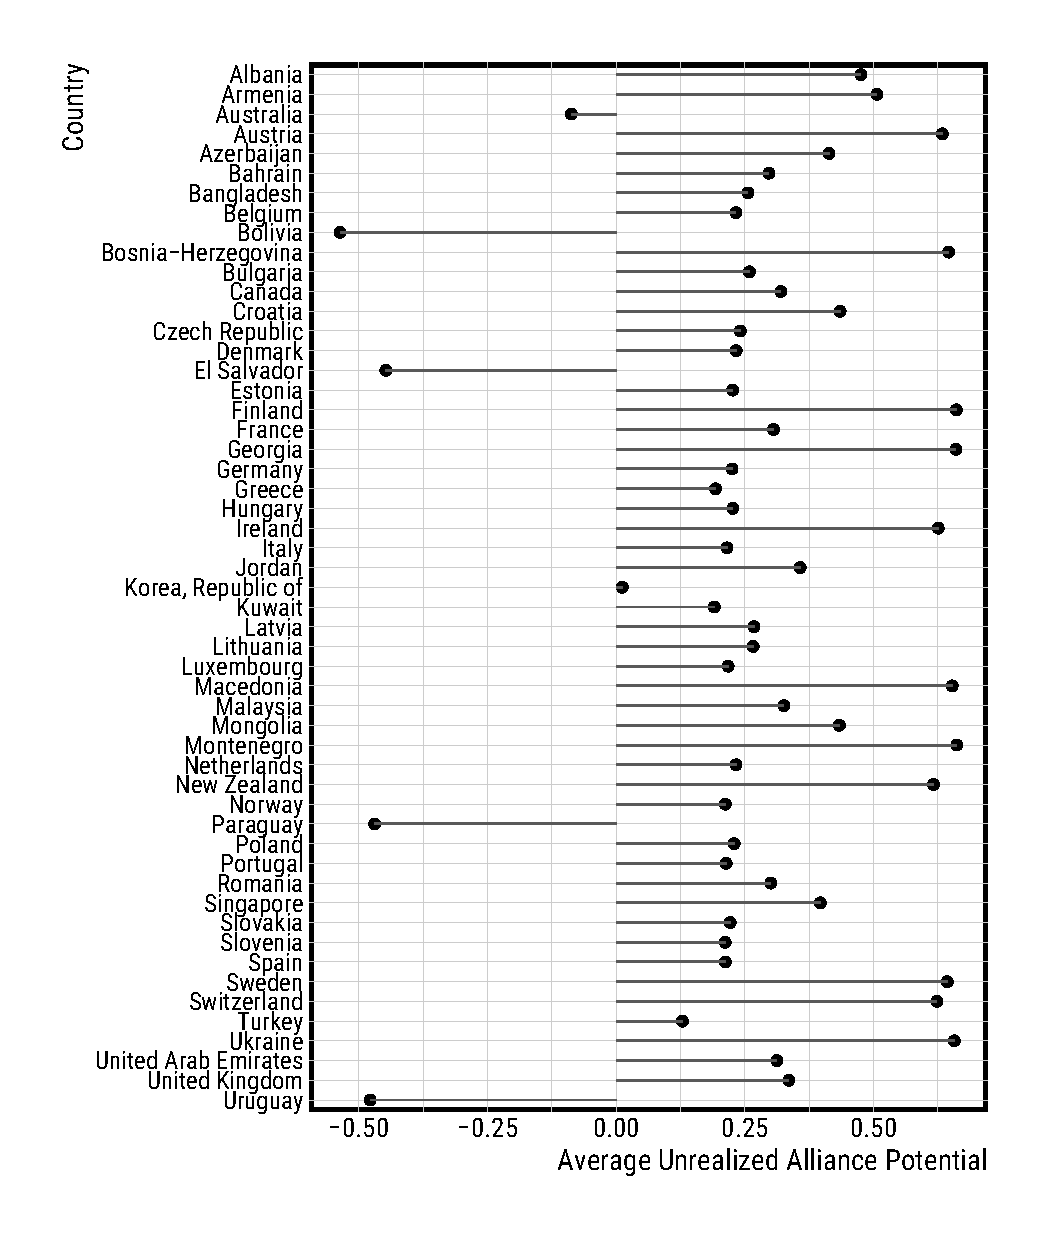
\includegraphics[height = 0.9\textheight]{figures/descriptive_stats.pdf}
				\caption{Unrealized alliance potential by countries that contributed troops. Unrealized alliance potential is our predictor of interest and represents whether a country's alliance with the United States is stronger or weaker than preferential estimates would suggest. The higher the value, then the more a state's alliance with the US is not as strong as it should be, given their preference alignment with the US.}
				\label{fig:measure_comparison_alliances}
			\end{center}
		\end{figure}

		We predict that states with a weaker relationship with the US than they desire are more likely to choose costly contributions to signal that dissatisfaction to the United States in the hopes that such a signal will curry favor and thus ``realize" the relationship's alliance potential. The earlier example comparing the UK, Venezuela, and New Zealand is illustrative of this concept. New Zealand represents an example of a state with security-based reasons for desiring a much stronger relationship with the United States, but one whose actual formal ties fall short. Unsurprisingly, New Zealand in turn makes incredibly costly contributions to the coalition. In contrast, contributions from states that are satisfied with their current relationship with the US (e.g. the UK or Venezuela) should be proportional to the strength of their current relationship rather than unexpectedly costly.
						
	\subsection{Model and Results}
		Our unit of analysis for these models is the country-year, spanning from 2001-2014. Our dependent variable for each model is the percent of a state's total troops contributed to Afghanistan annually. The primary predictor of interest operationalizes ``unrealized alliance potential" -- the difference between a country's United Nations voting similarity with the United States and the depth of its alliance with the United States. Because our theory is linear and our outcome is continuous we estimate a series of linear regressions. We also run a fixed effects model to check if the estimated effect of interest holds once we account for time-invariant unobserved confounders.

		The four categories of existing explanations for coalition warfare contribution -- collection action, balance of threat, alliance dependence, and domestic politics -- are used to identify a battery of proper control variables. We limit our model to these control variables in line with recommendations against ``garbage can" regressions \citep{ray_explaininginterstateconflict_2003, bleek_securityguaranteesallied_2014}. Existing theories suggest observable indicators of these variables are causally related and prior to the dependent and independent variables of interest.
		
		We include a measure of the Composite Index of National Capabilities (CINC) as well as economic measures of logged GDP and logged GDP per capita in line with the collective action hypothesis that the highest contributions should come from states with larger military and economic capacity because alliances are public goods \citep{olson_economictheoryalliances_1966, singer_capabilitydistributionuncertainty_1972}. Because the balance of threat hypothesis posits state contributions should be proportional to the gravity of the threat, we include a variable for geographic distance from Afghanistan to proxy for how likely a country is to be affected by instability and conflict in the region \citep{weidmann_geographyinternationalsystem_2010}. To account for changes in the perceived threat during the course of the conflict, we include lagged casualties since states experiencing casualties may consequently scale down their contributions. Because casualty aversion is closely associated with domestic explanations of coalition participation, this measure also accounts for theories about domestic determinants \citep{koch_casualtiesconstituenciesdemocratic_2005, jakobsen_denmarkafghanistanworth_2015}. Sine other domestic explanations are more broadly concerned with regime type, we include a control variable for whether a state is a democracy. For example, \citet{gartzke_democracypreparationwar_2001} and \citet{gartzke_whydemocraciesmay_2004} argue that democracies may be less reliable allies because high information costs and short leader tenure make commitments less guaranteed. To differentiate our explanatory variable from existing explanations of alliance dependence, we include variables for UN voting similarity and presence of an alliance with the United States \citep{bailey_estimatingdynamicstate_2017}. Current theories argue that troop contributions are most likely from a state's existing allies because you can leverage your relationship with allies to encourage contributions \citep{davidson_neoclassicalrealistexplanation_2011}. We expect these variables to have positive coefficients, but that unrealized alliance potential has explanatory power above and beyond when it comes to the amount of troops that states contributed.
		
		\newpage
		\begin{table}[H]
\begin{center}
\begin{tabular}{l c c c c }
\hline
 & Baseline & Political Controls & All Controls & Fixed Effects \\
\hline
Intercept      & $0.000^{*}$       & $0.002^{*}$         & $0.007^{*}$         &                     \\
               & $[0.000;\ 0.001]$ & $[0.001;\ 0.002]$   & $[0.002;\ 0.012]$   &                     \\
Potential Gain & $0.012^{*}$       & $0.014^{*}$         & $0.009^{*}$         & $0.010^{*}$         \\
               & $[0.011;\ 0.013]$ & $[0.012;\ 0.016]$   & $[0.006;\ 0.012]$   & $[0.003;\ 0.016]$   \\
Ideal Point    &                   & $0.002^{*}$         & $0.001^{*}$         & $-0.002^{*}$        \\
               &                   & $[0.001;\ 0.002]$   & $[0.000;\ 0.002]$   & $[-0.003;\ -0.000]$ \\
Democracy      &                   & $0.000$             & $0.000$             & $0.001$             \\
               &                   & $[-0.000;\ 0.001]$  & $[-0.001;\ 0.001]$  & $[-0.000;\ 0.002]$  \\
Casualties     &                   & $0.000^{*}$         & $0.000^{*}$         & $0.000^{*}$         \\
               &                   & $[0.000;\ 0.000]$   & $[0.000;\ 0.000]$   & $[0.000;\ 0.000]$   \\
U.S. Ally      &                   & $-0.003^{*}$        & $-0.001$            & $0.006^{*}$         \\
               &                   & $[-0.004;\ -0.002]$ & $[-0.002;\ 0.001]$  & $[0.001;\ 0.011]$   \\
CINC Score     &                   & $-0.020^{*}$        & $0.006$             & $-0.067$            \\
               &                   & $[-0.034;\ -0.006]$ & $[-0.011;\ 0.022]$  & $[-0.177;\ 0.042]$  \\
Log GDP        &                   &                     & $-0.001^{*}$        &                     \\
               &                   &                     & $[-0.001;\ -0.000]$ &                     \\
Log GDPPC      &                   &                     & $0.001^{*}$         &                     \\
               &                   &                     & $[0.001;\ 0.001]$   &                     \\
Distance       &                   &                     & $-0.000^{*}$        &                     \\
               &                   &                     & $[-0.000;\ -0.000]$ &                     \\
\hline
AIC            & -17677.705        & -13883.175          & -6404.655           &                     \\
BIC            & -17660.471        & -13839.153          & -6353.043           &                     \\
Log Likelihood & 8841.852          & 6949.587            & 3213.328            &                     \\
Deviance       & 0.064             & 0.050               & 0.016               &                     \\
Num. obs.      & 2309              & 1813                & 806                 & 1813                \\
R$^2$          &                   &                     &                     & 0.085               \\
Adj. R$^2$     &                   &                     &                     & -0.003              \\
\hline
\multicolumn{5}{l}{\scriptsize{$^*$ 0 outside the confidence interval}}
\end{tabular}
\caption{Statistical models}
\label{table:coefficients}
\end{center}
\end{table}

		\newpage

		As Table 1 demonstrates, regardless of model specification we find that the coefficient for potential gain with the United States is positive and statistically significant. Moreover, when these estimates are considered in terms of predicted contributions, then we see that a substantial amount of variation occurs. Expanding on the substantive meaning of this relationship, in figure \ref{fig:predict} we hold all covariates at their central values and then calculate how much a country's predicted troop contribution varies when the average unrealized alliance potential value (0.25) is shifted by one standard deviation in either direction. For the average-sized military -- 111,976 troops -- a one standard deviation change in unrealized alliance potential corresponds with a predicted difference of roughly 200 troops contributed to the ISAF coalition each year. This expected change becomes much greater for larger militaries and, inversely, lower for smaller militaries. If one considers the political costs of sending troops abroad, where even one casualty in another state's war can be politically disastrous, then it becomes apparent that these coefficient estimates are not just statistically significant, but politically meaningful. As mentioned, the 21 Dutch casualties in Afghanistan were sufficiently consequential that public outcry resulted in a vote that collapsed the government. The new government was forced to pull out of the war early, and as a result the broader coalition war efforts suffered a serious setback \citep[95-100]{massie_whydemocraticallies_2016}.

		\begin{figure}[p!]
			\centering
			\resizebox{1.05\linewidth}{!}{
				% Created by tikzDevice version 0.12 on 2020-05-12 17:36:37
% !TEX encoding = UTF-8 Unicode
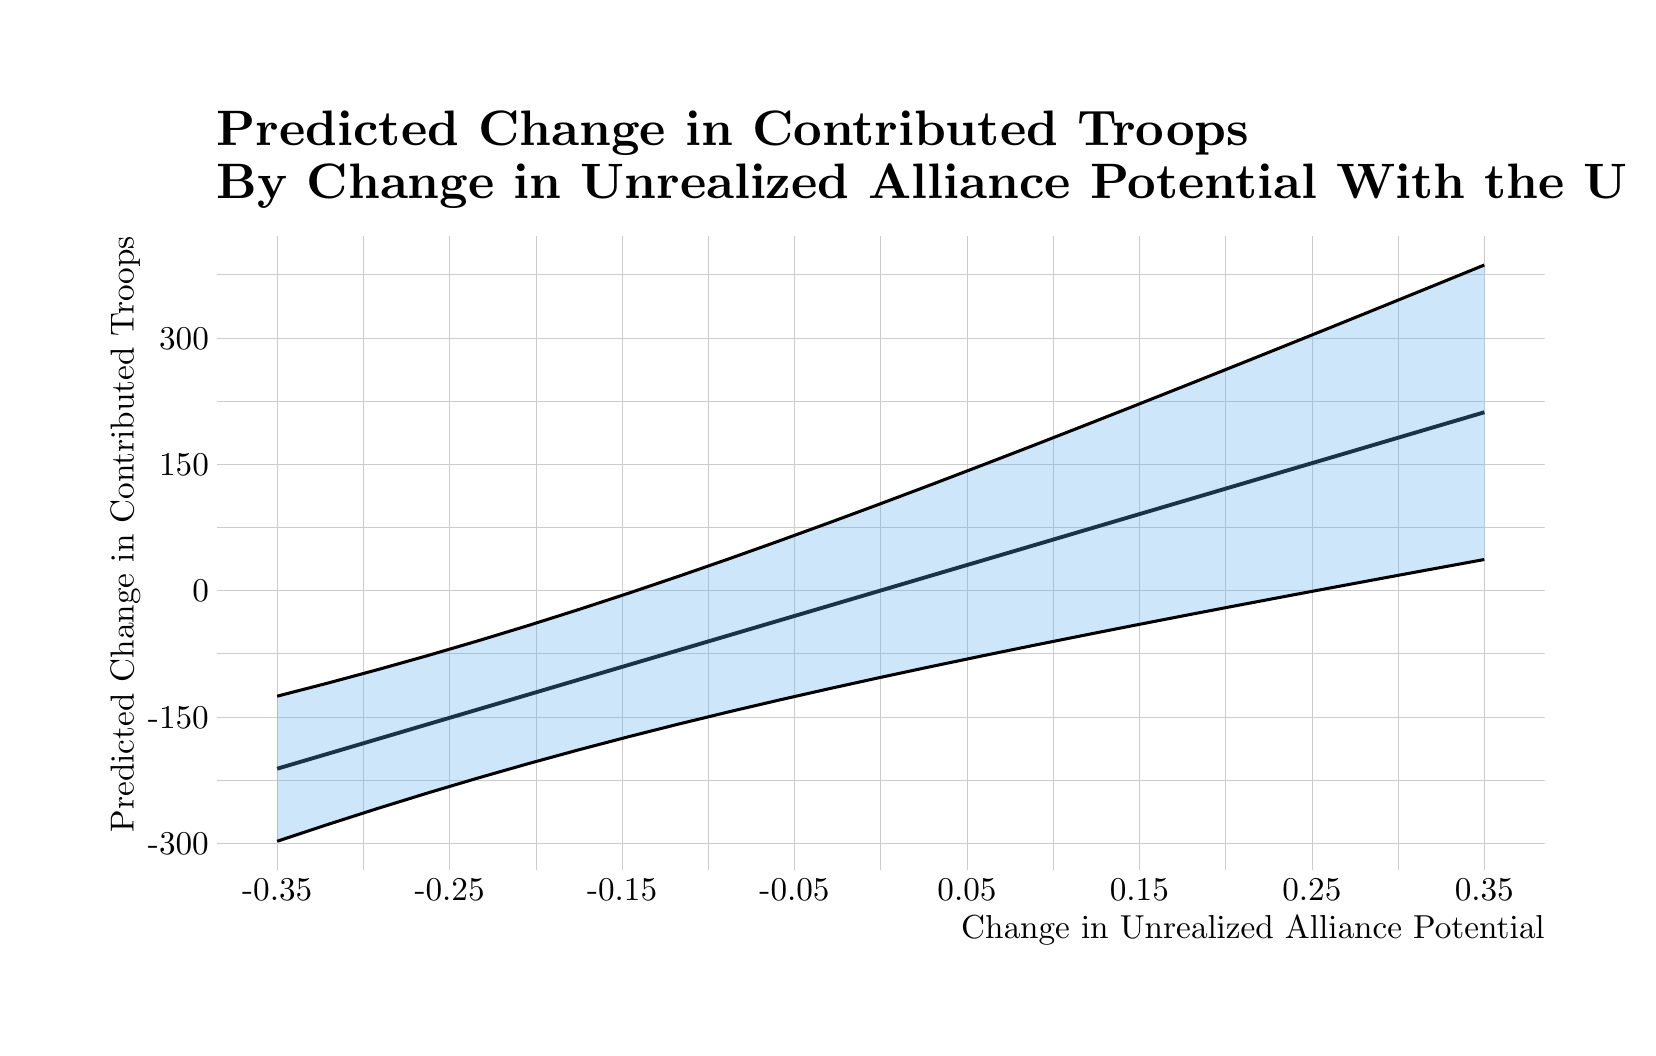
\begin{tikzpicture}[x=1pt,y=1pt]
\definecolor{fillColor}{RGB}{255,255,255}
\path[use as bounding box,fill=fillColor,fill opacity=0.00] (0,0) rectangle (578.16,361.35);
\begin{scope}
\path[clip] ( 68.34, 56.94) rectangle (548.16,285.99);
\definecolor{drawColor}{gray}{0.80}

\path[draw=drawColor,line width= 0.2pt,line join=round] ( 68.34, 89.49) --
	(548.16, 89.49);

\path[draw=drawColor,line width= 0.2pt,line join=round] ( 68.34,135.15) --
	(548.16,135.15);

\path[draw=drawColor,line width= 0.2pt,line join=round] ( 68.34,180.80) --
	(548.16,180.80);

\path[draw=drawColor,line width= 0.2pt,line join=round] ( 68.34,226.45) --
	(548.16,226.45);

\path[draw=drawColor,line width= 0.2pt,line join=round] ( 68.34,272.10) --
	(548.16,272.10);

\path[draw=drawColor,line width= 0.2pt,line join=round] (121.31, 56.94) --
	(121.31,285.99);

\path[draw=drawColor,line width= 0.2pt,line join=round] (183.62, 56.94) --
	(183.62,285.99);

\path[draw=drawColor,line width= 0.2pt,line join=round] (245.94, 56.94) --
	(245.94,285.99);

\path[draw=drawColor,line width= 0.2pt,line join=round] (308.25, 56.94) --
	(308.25,285.99);

\path[draw=drawColor,line width= 0.2pt,line join=round] (370.57, 56.94) --
	(370.57,285.99);

\path[draw=drawColor,line width= 0.2pt,line join=round] (432.88, 56.94) --
	(432.88,285.99);

\path[draw=drawColor,line width= 0.2pt,line join=round] (495.19, 56.94) --
	(495.19,285.99);

\path[draw=drawColor,line width= 0.2pt,line join=round] ( 68.34, 66.67) --
	(548.16, 66.67);

\path[draw=drawColor,line width= 0.2pt,line join=round] ( 68.34,112.32) --
	(548.16,112.32);

\path[draw=drawColor,line width= 0.2pt,line join=round] ( 68.34,157.97) --
	(548.16,157.97);

\path[draw=drawColor,line width= 0.2pt,line join=round] ( 68.34,203.62) --
	(548.16,203.62);

\path[draw=drawColor,line width= 0.2pt,line join=round] ( 68.34,249.27) --
	(548.16,249.27);

\path[draw=drawColor,line width= 0.2pt,line join=round] ( 90.15, 56.94) --
	( 90.15,285.99);

\path[draw=drawColor,line width= 0.2pt,line join=round] (152.47, 56.94) --
	(152.47,285.99);

\path[draw=drawColor,line width= 0.2pt,line join=round] (214.78, 56.94) --
	(214.78,285.99);

\path[draw=drawColor,line width= 0.2pt,line join=round] (277.09, 56.94) --
	(277.09,285.99);

\path[draw=drawColor,line width= 0.2pt,line join=round] (339.41, 56.94) --
	(339.41,285.99);

\path[draw=drawColor,line width= 0.2pt,line join=round] (401.72, 56.94) --
	(401.72,285.99);

\path[draw=drawColor,line width= 0.2pt,line join=round] (464.04, 56.94) --
	(464.04,285.99);

\path[draw=drawColor,line width= 0.2pt,line join=round] (526.35, 56.94) --
	(526.35,285.99);
\definecolor{drawColor}{RGB}{0,0,0}

\path[draw=drawColor,line width= 1.4pt,line join=round] ( 90.15, 93.57) --
	(108.33, 98.93) --
	(126.50,104.30) --
	(144.68,109.67) --
	(162.85,115.03) --
	(181.03,120.40) --
	(199.20,125.77) --
	(217.38,131.14) --
	(235.55,136.50) --
	(253.73,141.87) --
	(271.90,147.24) --
	(290.08,152.60) --
	(308.25,157.97) --
	(326.43,163.34) --
	(344.60,168.70) --
	(362.78,174.07) --
	(380.95,179.44) --
	(399.13,184.81) --
	(417.30,190.17) --
	(435.48,195.54) --
	(453.65,200.91) --
	(471.83,206.27) --
	(490.00,211.64) --
	(508.18,217.01) --
	(526.35,222.37);
\definecolor{fillColor}{RGB}{92,172,238}

\path[fill=fillColor,fill opacity=0.30] ( 90.15,119.78) --
	(108.33,124.48) --
	(126.50,129.38) --
	(144.68,134.49) --
	(162.85,139.82) --
	(181.03,145.36) --
	(199.20,151.12) --
	(217.38,157.07) --
	(235.55,163.22) --
	(253.73,169.53) --
	(271.90,176.01) --
	(290.08,182.62) --
	(308.25,189.35) --
	(326.43,196.19) --
	(344.60,203.13) --
	(362.78,210.14) --
	(380.95,217.23) --
	(399.13,224.38) --
	(417.30,231.58) --
	(435.48,238.82) --
	(453.65,246.11) --
	(471.83,253.43) --
	(490.00,260.79) --
	(508.18,268.17) --
	(526.35,275.58) --
	(526.35,169.17) --
	(508.18,165.84) --
	(490.00,162.49) --
	(471.83,159.11) --
	(453.65,155.70) --
	(435.48,152.26) --
	(417.30,148.77) --
	(399.13,145.24) --
	(380.95,141.65) --
	(362.78,138.00) --
	(344.60,134.28) --
	(326.43,130.48) --
	(308.25,126.59) --
	(290.08,122.59) --
	(271.90,118.47) --
	(253.73,114.21) --
	(235.55,109.79) --
	(217.38,105.20) --
	(199.20,100.42) --
	(181.03, 95.44) --
	(162.85, 90.25) --
	(144.68, 84.84) --
	(126.50, 79.22) --
	(108.33, 73.39) --
	( 90.15, 67.36) --
	cycle;

\path[] ( 90.15,119.78) --
	(108.33,124.48) --
	(126.50,129.38) --
	(144.68,134.49) --
	(162.85,139.82) --
	(181.03,145.36) --
	(199.20,151.12) --
	(217.38,157.07) --
	(235.55,163.22) --
	(253.73,169.53) --
	(271.90,176.01) --
	(290.08,182.62) --
	(308.25,189.35) --
	(326.43,196.19) --
	(344.60,203.13) --
	(362.78,210.14) --
	(380.95,217.23) --
	(399.13,224.38) --
	(417.30,231.58) --
	(435.48,238.82) --
	(453.65,246.11) --
	(471.83,253.43) --
	(490.00,260.79) --
	(508.18,268.17) --
	(526.35,275.58);

\path[] (526.35,169.17) --
	(508.18,165.84) --
	(490.00,162.49) --
	(471.83,159.11) --
	(453.65,155.70) --
	(435.48,152.26) --
	(417.30,148.77) --
	(399.13,145.24) --
	(380.95,141.65) --
	(362.78,138.00) --
	(344.60,134.28) --
	(326.43,130.48) --
	(308.25,126.59) --
	(290.08,122.59) --
	(271.90,118.47) --
	(253.73,114.21) --
	(235.55,109.79) --
	(217.38,105.20) --
	(199.20,100.42) --
	(181.03, 95.44) --
	(162.85, 90.25) --
	(144.68, 84.84) --
	(126.50, 79.22) --
	(108.33, 73.39) --
	( 90.15, 67.36);

\path[draw=drawColor,line width= 1.1pt,line join=round] ( 90.15, 67.36) --
	(108.33, 73.39) --
	(126.50, 79.22) --
	(144.68, 84.84) --
	(162.85, 90.25) --
	(181.03, 95.44) --
	(199.20,100.42) --
	(217.38,105.20) --
	(235.55,109.79) --
	(253.73,114.21) --
	(271.90,118.47) --
	(290.08,122.59) --
	(308.25,126.59) --
	(326.43,130.48) --
	(344.60,134.28) --
	(362.78,138.00) --
	(380.95,141.65) --
	(399.13,145.24) --
	(417.30,148.77) --
	(435.48,152.26) --
	(453.65,155.70) --
	(471.83,159.11) --
	(490.00,162.49) --
	(508.18,165.84) --
	(526.35,169.17);

\path[draw=drawColor,line width= 1.1pt,line join=round] ( 90.15,119.78) --
	(108.33,124.48) --
	(126.50,129.38) --
	(144.68,134.49) --
	(162.85,139.82) --
	(181.03,145.36) --
	(199.20,151.12) --
	(217.38,157.07) --
	(235.55,163.22) --
	(253.73,169.53) --
	(271.90,176.01) --
	(290.08,182.62) --
	(308.25,189.35) --
	(326.43,196.19) --
	(344.60,203.13) --
	(362.78,210.14) --
	(380.95,217.23) --
	(399.13,224.38) --
	(417.30,231.58) --
	(435.48,238.82) --
	(453.65,246.11) --
	(471.83,253.43) --
	(490.00,260.79) --
	(508.18,268.17) --
	(526.35,275.58);
\end{scope}
\begin{scope}
\path[clip] (  0.00,  0.00) rectangle (578.16,361.35);
\definecolor{drawColor}{RGB}{0,0,0}

\node[text=drawColor,anchor=base east,inner sep=0pt, outer sep=0pt, scale=  1.20] at ( 65.47, 62.54) {-300};

\node[text=drawColor,anchor=base east,inner sep=0pt, outer sep=0pt, scale=  1.20] at ( 65.47,108.19) {-150};

\node[text=drawColor,anchor=base east,inner sep=0pt, outer sep=0pt, scale=  1.20] at ( 65.47,153.84) {0};

\node[text=drawColor,anchor=base east,inner sep=0pt, outer sep=0pt, scale=  1.20] at ( 65.47,199.49) {150};

\node[text=drawColor,anchor=base east,inner sep=0pt, outer sep=0pt, scale=  1.20] at ( 65.47,245.14) {300};
\end{scope}
\begin{scope}
\path[clip] (  0.00,  0.00) rectangle (578.16,361.35);
\definecolor{drawColor}{RGB}{0,0,0}

\node[text=drawColor,anchor=base,inner sep=0pt, outer sep=0pt, scale=  1.20] at ( 90.15, 45.81) {-0.35};

\node[text=drawColor,anchor=base,inner sep=0pt, outer sep=0pt, scale=  1.20] at (152.47, 45.81) {-0.25};

\node[text=drawColor,anchor=base,inner sep=0pt, outer sep=0pt, scale=  1.20] at (214.78, 45.81) {-0.15};

\node[text=drawColor,anchor=base,inner sep=0pt, outer sep=0pt, scale=  1.20] at (277.09, 45.81) {-0.05};

\node[text=drawColor,anchor=base,inner sep=0pt, outer sep=0pt, scale=  1.20] at (339.41, 45.81) {0.05};

\node[text=drawColor,anchor=base,inner sep=0pt, outer sep=0pt, scale=  1.20] at (401.72, 45.81) {0.15};

\node[text=drawColor,anchor=base,inner sep=0pt, outer sep=0pt, scale=  1.20] at (464.04, 45.81) {0.25};

\node[text=drawColor,anchor=base,inner sep=0pt, outer sep=0pt, scale=  1.20] at (526.35, 45.81) {0.35};
\end{scope}
\begin{scope}
\path[clip] (  0.00,  0.00) rectangle (578.16,361.35);
\definecolor{drawColor}{RGB}{0,0,0}

\node[text=drawColor,anchor=base east,inner sep=0pt, outer sep=0pt, scale=  1.20] at (548.16, 32.33) {Change in Unrealized Alliance Potential};
\end{scope}
\begin{scope}
\path[clip] (  0.00,  0.00) rectangle (578.16,361.35);
\definecolor{drawColor}{RGB}{0,0,0}

\node[text=drawColor,rotate= 90.00,anchor=base east,inner sep=0pt, outer sep=0pt, scale=  1.20] at ( 38.26,285.99) {Predicted Change in Contributed Troops};
\end{scope}
\begin{scope}
\path[clip] (  0.00,  0.00) rectangle (578.16,361.35);
\definecolor{drawColor}{RGB}{0,0,0}

\node[text=drawColor,anchor=base west,inner sep=0pt, outer sep=0pt, scale=  1.80] at ( 68.34,318.93) {\bfseries Predicted Change in Contributed Troops };

\node[text=drawColor,anchor=base west,inner sep=0pt, outer sep=0pt, scale=  1.80] at ( 68.34,299.49) {\bfseries By Change in Unrealized Alliance Potential With the United States};
\end{scope}
\end{tikzpicture}

			}
			\caption{Predicted change in the number of contributed troops by change in unrealized alliance potential with the United States. The x-axis covers one standard deviation (0.35) in the observed unrealized alliance potential estimates, spanning from a country's alliance strengthening with the United States (negative values) to its alliance weakening (positive values). The y-axis is the predicted number of troops contributed for the average country with 95\% confidence intervals. For a single standard deviation change in a country's unrealized alliance potential we estimate an average increase or decrease of 200 contributed troops, with the expected magnitude increasing by a substantial amount for larger militaries.}
			\label{fig:predict}
		\end{figure}

% Qualitative evidence of our theory and the causal logic for New Zealand
		The results of the statistical model are supported by qualitative evidence demonstrating the salience of the cost of partner contributions in the minds of policymakers. US Secretary of Defense Gates noted during the war in Afghanistan that there was a ``two-tiered alliance" that made a distinction between ``allies willing to fight and die to protect people's security and others who are not" \citep[328]{ringsmose_natoburdensharingredux_2010}. New Zealand's prominence as an exemplary case is intentional. Their relationship with the United States began to sour in 1984 after disagreements over the effects of a nuclear weapon free zone on US ship movements caused a split in ANZUS \citep{catalinac_whynewzealand_2010}. The relationship continued to decline after New Zealand Prime Minister Helen Clark publicly opposed the Iraq War, a stance that kept New Zealand on the sidelines while the US negotiated new trade talks with Australia \citep{armstrong_alliesrewardedtrade_2003}. New Zealand's decision to over-contribute to US efforts in Afghanistan may have been a way to shore up relations that New Zealand felt should be strong given the two states see eye to eye on most international affairs. Interviews of New Zealand government and military officials conducted by \citet{wellings_narrativealignmentmisalignment_2018} noted participation in Afghanistan was a way for New Zealand to ``punch above its weight" militarily. Almost all New Zealand's Provincial Reconstruction Teams (PRTs) were deployed in Regional Command-East which was headed by the United States \citep[49]{auerswald_natoafghanistanfighting_2014}, allowing them to ``rub shoulders with countries that we couldn't normally" \citep{wellings_narrativealignmentmisalignment_2018}. New Zealand believed an improved relationship with the US would have longer term geopolitical pay-offs, with one former defense official noting ``we all had those credentials of working with the US\ldots After a while they plugged in that the Americans trust us" \citep[31]{wellings_narrativealignmentmisalignment_2018}. They thus saw participation in the war as a way of sending a costly signal; a way to ``rejuvenate" their security relationship with the US \citep[128]{burton_natodurabilitypostcold_2018}.
		
% Qualitative evidence of our theory and the causal logic for Norway		
		Similar evidence has been observed with Nordic states who made costly contributions to improve their relationship with the US because they believed a stronger relationship would improve their international status \citep{pedersen_bandwagonstatuschanging_2018}. Norway justified their contributions to Afghanistan based on the potential benefits of unrealized alliance improvements \citep{oma_smallstatesburdensharing_2014}. While initially asked to simply contribute peacekeepers to the UN humanitarian mission, Norway's Ministry of Defence felt that was not a sufficient demonstration of their support for the US-led operation \citep{ministryofdefenceiisecuritypolicy_mulignorskubatstotte_2001}. The Ministry of Defence wrote a memorandum to the Norwegian government expressing its concern that the absence of a noteworthy military contribution would ``pose problems for Norway's security relations with the US" and that the nation would benefit from showing it is ``able and willing to make relevant contributions" \citep{ministryofdefenceiisecuritypolicy_muligenorskemilitaere_2001}. Not only was an improved relationship with the United States an explicit motivation for Norway's participation in Afghanistan, it justified a military troop contribution because of the signal Norway felt that would send to the United States. In the Ministry of Defence's official public report on Norway's participation in Afghanistan, they noted that ``the US authorities saw participation in the military operations as the most important means by which other countries could demonstrate their support for the `war on terror' and for promoting a stable Afghanistan\ldots Demonstrating to Washington and Brussels that Norway was a capable contributor was more important in Norwegian decision-making than assessments of the potential effects Norway's relatively small contributions would have in Afghanistan" \citep[214-216]{godal_goodallynorway_2016}.
		
		We take caution in noting that alliance considerations are clearly not the sole factor motivating a state's decision about how much to contribute to coalition conflicts. Although \citet{mello_pathscoalitiondefection_2020} considers a different situation -- looking at a state's contribution over the course of a conflict and their decision to withdraw support based on domestic considerations -- the salience of domestic factors in motivating decisions about how much to contribute is worthy of note. Situations like the domestic backlash that forced Latvian withdrawal from Iraq after the death of two soldiers identifies why over-contributions can be costly signals of a state's desire for a stronger alliance relationship; these contributions carry domestic political risks that also factor prominently in calculations about how many troops to contribute to coalition efforts.

\section{Implications}
	Because alliance membership is a club good, not a pure public good, worries about being excluded from the security benefits of an alliance can incentivize a state to try to shore up the alliance by sending a costly signal of their commitment to their alliance partners. ``Today, we should expect the European allies to find that the best way to strengthen (or avoid weakening) their bonds with the United States is to contribute to out-of-area operations like ISAF. According to this line of reasoning, the allies who put the highest premium on NATO’s traditional products should be the ones – together with the United States – shouldering the heaviest burdens in Afghanistan" \citep[331]{ringsmose_natoburdensharingredux_2010}. Yet the Afghanistan case demonstrates this is not just a story about formal NATO membership, but security cooperation more generally. States may use war efforts as a signal of their willingness to accept large costs in the hopes that this will improve their relationship with the coalition leader in the future. This helps explain the ways that states use conflicts that are not of immediate strategic importance to -- hopefully -- gain the attention and respect of important actors in the international system.

	Closer alignments may be valued inherently, for unspecified reasons, or to help the state acquire side payments or policy concessions on unrelated issues. \citet{henke_buyingalliespayment_2019} argues that states contribute to coalition conflicts when the ``pivotal state" -- what we call the coalition leader -- provides side payments as incentives to contribute. This highlights our broader logic about variation in club goods and public goods in alliances and coalitions. States contribute to coalition warfare when there are benefits to contributing troops that fall outside the traditionally understood alliance mandates or security concerns. In US-led conflicts since the Korean War, \citet{henke_buyingalliespayment_2019} find that future benefits offered by pivotal states can induce coalition participation. We extend upon this finding by arguing that the states most likely to be moved by that logic are those with unrealized alliance potential. Furthermore, they will go above and beyond in their coalition participation to try to secure future benefits -- whether side payments or unrelated payments -- that extend from a closer relationship with the coalition leader. Thus, desire for stronger ties and the expectation that over-contribution will positively signal that desire explains our findings in a way that run counter to previous theories.
	
	Our findings run counter to predictions from theories concerning the balance of threats \citep{walt_originsalliance_1987}. For the balance of threat hypothesis, the states with the highest contributions are those that are most concerned about the threat the opposing state presents to their security \citep{haesebrouck_democraticparticipationair_2016}. Yet, when contributions are measured as internal costs relative to the contributions a state could have made, the highest contributions are from states that appear to be opting into a war in which they have no material stake. Denmark, New Zealand, and Romania, 3 of the top 4 contributors to ISAF in 2001 by our measure, are not the states that are most concerned about the threat that the Taliban and Al-Qaeda posed to their national security.

	Previous theories described under the rubric of the alliance hypothesis also fail to explain this finding. For previous theories, ally support is expected when you can leverage your allies' power in your favor and is thus positively associated with closeness \citep{davidson_neoclassicalrealistexplanation_2011, massie_democraticalliesfollowership_2016}. This expects the closest US allies to be the largest contributors to US war efforts. Yet the relationship we see does not follow this trend. States do not over-contribute because the United States is their best protector or because they think they have the ability to influence the United States through their international clout as \citet{ringsmose_natoburdensharingredux_2010} posits. States with a strong but stable current alliance have fewer incentives to over-contribute because they don't get any additional payoff from doing so and there is little risk of fallout from a normal or small contribution because the alliance is already strong \citep{davidson_headingexitsdemocratic_2014}.
	
	Rather, it is the states that \textit{want} the United States to be their best protector or that \textit{want} the ability to influence international relations with the United States that are most likely to over-contribute \citep{vonhlatky_greatasymmetryamerica_2010}. This is why small states are able to free ride and take the relationship for granted as pointed out by \citet{keohane_biginfluencesmall_1971}, but we don't always see this because states that desired an improved tie will in fact try to signal that they are not free riders. Rather, acquaintances that do benefit from signaling a change in their desired alignment tie will undertake more intense participation \citep{gibler_priorcommitmentscompatible_2004, gartzke_contractsfriendsalliances_2012}. Canada, for example, was concerned about accusations of free riding on the US alliance and thus intensified their participation in Afghanistan to elevate their status in the eyes of American policymakers \citep{massie_alliancevaluestatus_2018}. If the US-Canada relationship had already been sufficiently strong, there would have been a reduced need to signal their value to the relationship. It is also not the case that the US coerced its closest allies into participating as argued by \citet{kupchan_natopersiangulf_1988} because those are not the states that ended up doing the most participating relative to what they could have contributed. And while NATO membership and its accompanying obligations may be sufficient to explain why states do not free ride or defect, that does not explain why states not bound by alliance obligations (eg. New Zealand) end up over-contributing.

	This points to the importance of understanding who joins military coalitions and why \citep{wolford_politicsmilitarycoalitions_2015, moller_fightingfriendsinstitutional_2016}. The quality of a coalition impacts factors like military skill, coordination, and legitimacy \citep{kreps_coalitionsconvenienceunited_2011, auerswald_natoafghanistanfighting_2014, saideman_ambivalentcoalitiondoing_2016, cranmer_coalitionqualitymultinational_2017, cappellazielinski_organizingperformancecoalition_2020}. But having more eager partners is not always an obvious gain. Receiving coalition support from acquaintances rather than close allies could reduce the ease of coordination and increase the cost of side payments \citep{morrow_alliancesasymmetryalternative_1991, papayoanou_intraalliancebargainingbosnia_1997, wolford_politicsmilitarycoalitions_2015, henke_buyingalliespayment_2019}. During the Korean War, for example, the United States turned down Pakistan's offer of coalition forces due to fears of operational inefficiency and a loss of US control over battlefield decisions \citep{stueck_koreanwarinternational_1997}. Unanticipated defection by partners that initially joined Operation Iraqi Freedom similarly increased expenses for those that remained \citep[12-13]{mcinnis_varietiesdefectionstrategies_2018}. It can also prove costly for the participating countries since engagement in overseas conflict impacts factors like public opinion and, ultimately, whether a politician remains in office \citep{chiozza_leadersinternationalconflict_2011, wolford_nationalleaderspolitical_2016, mello_pathscoalitiondefection_2020}. It bears repeating that the Netherlands' participation in the war in Afghanistan -- and its attendant 21 casualties -- is widely regarded as the primary reason for the government's collapse in 2010 \citep[152-156]{auerswald_natoafghanistanfighting_2014}.

	Our theory concerns whether an interest in a stronger relationship with the coalition leader influences the nature of a state's participation in a conflict; it does not seek to explain why a state may want a stronger relationship. Consequently, theories about the domestic determinants of coalition contributions are not competing explanations with the theory proposed here. Domestic factors could be the reason a state wants to establish itself as a closer ally with a powerful country \citep{tago_whenaredemocratic_2009, pilster_aredemocraciesbetter_2011, wolford_nationalleaderspolitical_2016} or otherwise impact coalition warfare participation \citep{baum_iraqcoalitionwilling_2013}. The domestic origins of alliance-motivated coalition contributions have been witnessed in Egypt in the 1960's \citep{barnett_domesticsourcesalliances_1991}, the United Kingdom during the Iraq War \citep{davidson_americaallieswar_2011}, and Canada since the war in Afghanistan \citep{massie_alliancevaluestatus_2018, mckay_whycanadabest_2018}. In these cases, political leaders who fear domestic opposition from other government actors like bureaucrats or non-partisans or from non-government actors like voters or interest groups may use alliances with other states to demonstrate competent policymaking. The reasoning behind a state's motivation for signaling their interest in a closer interstate relationship represents an important area of future research.

% Qualitative evidence of our theory and the causal logic for Norway and Denmark and Estonia
	Over over-contributions rewarded? Our findings do not present a clear answer, but that is not our goal. We argue only that states are making a strategic bet based on their belief that an over-contribution increases the probability of a stronger alliance. Whether this strategic bet pays off concerns the consequences of coalition warfare contributions; our theory is about its causes. While our finding suggests that state behavior is consistent with this calculated bet, the outcome of that bet is a different question. A dominant state, in this case the United States, need not strengthen their relationship with a state that over-contributed its armed forces. Evidence exists about contemporary instances of over-contributions helping states secure deeper security \citep{slavin_buildswarcoalition_2003} and economic ties \citep{whitmore_uswarallies_2003}, but more skeptical research about the ability to secure future benefits \citep{porter_lastchargeknights_2010} provides an avenue for future work investigating whether this strategic logic pays off; does the costly signal of over-contribution result in a closer alliance relationship?
			
	Nonetheless, the Afghanistan case provides suggestive evidence that states do reward over-contributions, possibly hoping that doing so will incentivize future over-contributions by other states. US Secretary of Defense Robert \citet{gates_securitydefenseagenda_2011} commended Denmark for its costly contribution to the conflict when he publicly noted that Denmark ``\ldots with their constrained resources, found ways to do the training, buy the equipment, and field the platforms necessary to make a credible military contribution." Importantly, it was not just that Denmark participated, but that they participated in a costly manner given their limited resources, that gained them accolades from the US Secretary of Defense. A high-ranking Danish official noted ``Danish market value in Washington soared as a result of Iraq and Afghanistan" \citep{henriksen_whatdiddenmark_2012}. The head of the British effort in southern Afghanistan, Brig. Cowan, similarly noted ``Denmark and Estonia are small countries but they're doing great things for the coalition. Estonia has been a staunch ally of America and Britain and they have sacrificed a lot of soldiers in this campaign" \citep{druzin_tinyestoniakeen_2009}. Countries with unexpectedly high contributions to the Iraq war -- eg. Australia, Poland, and Singapore -- received similar praise from the United States. US President George W. Bush described Australian Prime Minister John Howard as ``kind of like a Texan" during his invitation to Bush's Texas ranch; an invitation (also extended to Poland) that former national security adviser James Steinberg claimed places one in ``the first rank of America's friends" \citep{sanger_meanwhilebackranch_2003}.
	
	But the rewards of over-contributions are not just limited to verbal praise and ranch visits. The relationship between coalition contributions and policy concessions on economic cooperation has also been systematically documented \citep{long_tradingsecuritymilitary_2006}. At the outset of the Iraq War, both Chile and Singapore were engaged in initial discussion with the US over new bilateral free trade pacts. Singapore contributed troops to the Iraq War while Chile openly opposed it. At the signing of the new trade pact with Singapore, President Bush described Singapore as ``a strong partner in the war on terrorism and a member of the coalition on Iraq" \citep{armstrong_alliesrewardedtrade_2003}. Chile, on the other hand, had their free trade pact delayed, with US Trade Representative Zoellick noting ``I'm disappointed\ldots We worked very closely with our Chilean partners. We hoped for their support in a time we felt was very important". While Zoellick was not explicit in linking a lack of support in Iraq with the delay of closer trade relations, Chilean ambassador Andres Bianchi was, saying ``[t]o be absolutely honest, the signing of the agreement has been influenced by our decision at the Security Council" \citep{armstrong_alliesrewardedtrade_2003}. In this case, the benefits extended beyond side payments and instead concerned seeking policy concessions on unrelated issues.

% Qualitative evidence of our theory and the causal logic for non-ISAF wars (Libya, Iraq, and Sardinia)
	While our statistical analysis is limited to an examination of the war in Afghanistan, there is suggestive evidence that the theory holds for other coalition conflicts like US-led operations in Libya and Iraq, as well as less similar cases like the Crimean War. Norway's relationship with the US had soured since its early withdrawal from the Iraq war, resulting in an 8 year drought in bilateral meetings between the two heads of state \citep{jakobsen_europeannatoreally_2018}. During the later war in Libya, Norway made concerted efforts to over-contribute forces, particularly in the aerial bombing campaign, in order to demonstrate their ``relevance and trustworthiness to its great power allies in NATO, especially the United States" \citep[109]{jakobsen_goodnewslibya_2012}.\footnote{A detailed account of Denmark during the war in Libya is provided by \citet{dicke_natoburdensharinglibya_2013} and \citet{jakobsen_prestigeseekingsmallstates_2018}.}

	Even as far back as the 1850's, Sardinia's participation in the Crimean War exemplifies the logic of coalition contributions to improve alliance relationships \citep[17-25]{blumberg_carefullyplannedaccident_1990}. Knowing it could not defeat the Austrian Empire single-handed, Sardinia sought to curry favor with Napoleon III of France with the hopes it would gain support for expansion. To do so, Sardinia joined the French side during the Crimean War despite facing high domestic costs from the resulting casualties and increased taxation \citep[326]{gorce_histoiresecondempire_1902}. Sardinia's gamble was successful, as their participation in France's war against the Russian Empire was recognized with Napoleon III writing to Sardinian King Victor Emmanuel ``[y]our Majesty can also surely count on me as a true friend" \citep[1]{boselli_napoleoniiivictor_1926}. Historians have noted ``there is no doubt that Piedmont's diplomatic profile grew as a result of her involvement in the Crimean War and the seeds were sown for the deal agreed between Cavour and Napoleon III at Plombi\`{e}res on 20 July 1858." \citep{rathbone_piedmont1850s_2008}.

\section{Conclusion}
	A state's closest allies will not be the states most invested in fighting alongside that state. Rather, weakly aligned states that desire a closer relationship are most likely to over-contribute forces to coalition warfare. This finding produces a different list of contributors than what current theories predict. The study of state contributions to coalition warfare provides unique insights if those contributions are measured relative to the cost they impose onto the contributor rather than the utility they provide regarding the conflict outcome. Not every state contributes to a war effort in order to influence the outcome of the war as theories of balance of threats predict. But it is also not the case, as predicted by the collective action hypothesis that states simply free ride when the conflict outcome is immaterial or, as predicted by the alliance dependence hypothesis, that the stronger your alliance, the more you contribute.

	Rather, because war is costly, it can serve as a signaling function for states that want to convey their desire to improve their relationship with other states in the international system. By accepting comparatively large costs to fighting alongside another state, especially when such fighting does not otherwise benefit you, states can signal how much they value an alliance relationship in a way that they anticipate will generate reciprocity and payoffs down the road. Future work should examine whether states are making a smart bet in anticipating future payoffs from costly over-contributions; it is possible their gamble is incorrect. But for now, it suffices to say that states with the most interest in future payoffs from a better alliance relationship are the same states most likely to separate themselves from the rest of the coalition pact by over-contributing to wartime coalitions in the hopes that doing so signals their reliability.

\newpage

\theendnotes

\newpage

\bibliographystyle{apsr}
\bibliography{isaf_alliances}

\end{document}